\section{Serial Method}
In this section, the serial implementation of FTCS method is discussed. First the given PDE is decretized, and the initial and boundary conditions are specified. The stabilty condition is briefly touched to give reasoning on how to choose the step-sizes. Finally, the python program is revealed along with the results.
\subsection{Domain Discretization}
The numerical method that will be implemented to solve the given (1+1)-Dimensional Pure-Diffusion Equation is the FTCS (Forward Time Central Space) method. The given equation \autoref{eq:De} is discretized into \autoref{eq:Disceq}. Based on the centered space, symmetric finite differences for the space derivative was used (step-size in space $h/2$); and forward finite difference for the time derivative was used (step-size in time $\tau$).

\begin{equation}
\begin{aligned}
    v(x,t+\tau) = &v(x,t) \\
     &+ \dfrac{\tau}{h^2}D(x+h/2)[v(x+h,t) - v(x,t)] \\
     &+ \dfrac{\tau}{h^2}D(x-h/2)[v(x-h,t) - v(x,t)] \\
     &+ \tau S(x,t)
\end{aligned}
\label{eq:Disceq}
\end{equation}

The discretized domain is shown in \autoref{fig:DescretizedDomain}. This is a discretization of the same rod shown in \autoref{fig:Rod}. Note that in both figures, the centre of our 1D domain is placed at the origin $O$. With each far end of the domain being $L$ units from the origin. Each discretized cell is $h$ units.
\figDescretizedDomain

\subsection{Boundary and Initial Conditions}
\label{subsec:bic}
A key necessity to solving PDEs is the boundary and initial condition, here we use the Neumann boundaries: by setting $D(x)=0$ on the boundaries, i.e. $D(-L-h/2)=D(L+h/2)=0$ as shown in \autoref{fig:BorderDD}. The initial condition $v(x,t=0)=v_0$, $D(x)$, $S(x,t)$, the simulation time $T$ and domain length $2L$, can be given by the user in the program.

\figBorderDD

\subsection{Solution Matrix}
In order to plot the results, the value of each discretized cell ($x+h$) at each time-step ($t+\tau$) needs to be stored in solution matrix.

In our case, the solution matrix is a 2D matrix as shown in \autoref{fig:SolutionMat}, with each element representing the value of the scalar quantity $v$ at a particular time $\tau$ and space $h$. In the solution matrix, the rows represent the time-step $\tau$, and the columns represent the space-step $h$. The size of the matrix is dependent on the coarseness of the discretization. However, the domain of our solution will always be $x=[-L,L]$ and $t=[0,T]$.

\figSolutionMat

The implementation of discretizing the space and allocating the solution matrix in Python is shown below. Note that the boundaries, i.e. $-L-h$ and $L+h$ are included as well.

\begin{lstlisting}[language=Python]
# decretized space
x = np.linspace(-L-h,L+h, np.ceil(2*L/h).astype('int')+2)
N = int(T/tau)
# solution matrix including L-h/2 and L+h/2
V = np.zeros([N, np.size(x)]);
\end{lstlisting}

\subsection{Stability Condition}
The step-sizes, $h$ and $\tau$ are chosen such that accumulation of errors is prevented and the method is numerically stable. Thus we look into the stability condition. For the FTCS method of a 1D Parabolic PDE of the form $\frac{\partial u(x, t)}{\partial t} = \alpha \frac{\partial^2 u(x, t)}{\partial x^2}$, the following condition must be satisfied \cite{griffiths}.
\begin{equation}
    \dfrac{\tau}{h^2} \leq \dfrac{1}{2 \alpha}
    \label{eq:Stabilitycondition}
\end{equation}

In our given differential equation, there's no scalar coefficient, hence, $\alpha=1$. By fixing the value of $\tau$, we can then determine the least step-size $h$, and hence the maximum number of discretized cells in our domain, i.e. columns of the solution matrix, is also determined.

\vspace{1mm}
\textbf{Example:} Let us fix $\tau = 0.001$, and determine the minimum value for $h$ and the corresponding number of discretized cells. Continuing from \autoref{eq:Stabilitycondition}. 


\begin{equation}
    \begin{aligned}
        h&\geq\sqrt{2\tau} \\
        h&\geq\sqrt{2\cdot 0.001} \\ 
        h&\geq\frac{\sqrt{5}}{50} \quad (\text{where } \frac{\sqrt{5}}{50} \approx 0.0447)
    \end{aligned}
    \label{eq:Min_h}
\end{equation}
We can now determine the appropriate number of discretized cells of our domain ($\text{\#cols}$). Using the inequality obtained from \autoref{eq:Min_h} into the relationship $h = \frac{2L}{\text{\#cols}}$ from \autoref{fig:SolutionMat}.
\begin{equation}
    \begin{aligned}
        \frac{2L}{\text{\#cols}} &\geq \frac{\sqrt{5}}{50} \\
        \text{\#cols} &\leq \frac{2\cdot5}{\sqrt{5}/50}\\
        \text{\#cols} &\leq 100\sqrt{5} \quad (\text{where } 100\sqrt{5} \approx 223.6)
    \end{aligned}
\end{equation}
The similar approach can be done for finer values as well, \autoref{tab:Coarsness} below shows the values for $h$ and \#cols for various $\tau$ values.
\begin{table}[H]
    \centering
    \renewcommand{\arraystretch}{1.5}
    \begin{tabular}{|c|c|c|}
        \hline
        For $\tau = 1\times10^{-1}$ & $h \geq 0.1414$ & $\text{\#cols}\leq70.7$ \\
        \hline
        For $\tau = 1\times10^{-2}$ & $h \geq 0.0447$ & $\text{\#cols}\leq223.6$ \\
        \hline
        For $\tau = 1\times10^{-3}$ & $h \geq  0.0141$ & $\text{\#cols}\leq707.1$ \\
        \hline
        For $\tau = 1\times10^{-4}$ & $h \geq  0.0044$ & $\text{\#cols}\leq2236.1$ \\
        \hline
    \end{tabular}
    \caption{$\tau$ and $h$ that satisfy the stability condition \autoref{eq:Stabilitycondition}, and the corresponding \#cols for the solution matrix (i.e. the number of discretized cells in space) }
    \label{tab:Coarsness}
\end{table}

It should be noted that the size of the entire solution matrix would increase pretty quickly with finer values of $\tau$ or $h$. For our demonstration, we will henceforth only work with $\tau = 0.001$ and $\tau=0.0001$.

\subsection{Python Program (Serial)}
The following section will solve the FTCS method using a single processor. The parameters $2L$ for the domain length and $T$ for the simulation time are specified. The desired coarseness $h$ is chosen based on the value of $\tau$ and in accordance with the stability condition \autoref{eq:Stabilitycondition}. The program is run for two cases $\tau = 0.001$ and $\tau=0.0001$ respectively. The following parameters are fixed for each case:

\begin{table*}[h]
    \renewcommand{\arraystretch}{1}
\begin{tabular}{rl}
    $2L =$&$10$ \\
    $T =$&$2$ \\
    $h =$&$2L/\text{cols}$
\end{tabular}
\end{table*}

Thus specifiying our domain to $-5\leq x \leq 5$ and $0\leq t \leq 2$. Next, $\tau$ and $h$ are chosen based on the information from \autoref{tab:Coarsness}.
\begin{table*}[h]
    \centering
    \renewcommand{\arraystretch}{1}
\begin{tabular}{l|l}
    \textbf{case 1}  & \textbf{case 2} \\ 
    $\tau = 0.001$ & $\tau = 0.0001$\\
    cols = 223 $\implies$ $h=0.0448$  & cols = 707 $\implies$ $h=0.0141$
\end{tabular}
\end{table*}


\vspace{1mm}
The initial condition
$v_0 = 
\begin{cases}
1 & \text{if } |x|<1.5 \\
0 & \text{else }
\end{cases}
$. $D$ and $S$ are initialized as
\begin{lstlisting}[language=Python]
v0 = lambda x   : float(abs(x)<1.5);
D  = lambda x   : 1 
S  = lambda x,t : 0 
\end{lstlisting}

The numerical method begins by assigning the initial values in the solution matrix \texttt{V}.
\begin{lstlisting}[language=Python]
for l in range(np.size(x)):
    V[0,l] = v0(x[l])
\end{lstlisting}

The following code is the FTCS method. This is the direct translation of the discretized equation \autoref{eq:Disceq} to Python. The variables \texttt{Dp} and \texttt{Dm} represent the value of the coefficient $D(x)$ evaluated at $D(x+h/2)$ and $D(x-h/2)$, and it is $D(x) = 0$ at the borders as discussed in \autoref{subsec:bic}.

\begin{lstlisting}[language=Python]
for lt in range(1,N):
    for lx in range(1,np.size(x)-1):
        # evaluate D at lx
        Dp = D(x[lx]+h/2) * (np.abs(x[lx]+h/2)<L)
        Dm = D(x[lx]-h/2) * (np.abs(x[lx]-h/2)<L)

        V[lt,lx] = V[lt-1,lx] + (tau/h**2)*Dp*((V[lt-1,lx+1]) - V[lt-1,lx])+\
                                (tau/h**2)*Dm*((V[lt-1,lx-1]) - V[lt-1,lx])+\
                                tau*S(x[lx], -(lt-1)*tau)
\end{lstlisting}
From the for-loops, we can see that to evaluate \texttt{V} at every step in \texttt{lt} i.e. \texttt{V[lt,lx]}, the values of \texttt{V} at locations \texttt{lx-1, lx, lx+1} from the previous time-step \texttt{lt-1} must be known as shown in \autoref{fig:Graphftcs}.

\graphftcs

\subsection{Program Files}
The directory \texttt{serial\_diffusion} contains files to run the program as shown in \autoref{fig:Serialdir}. To run, execute the command: \texttt{\$ python main.py}.
\begin{figure}[H]
    \centering
    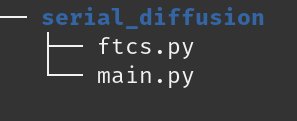
\includegraphics[width=0.3\textwidth]{figures/serial_dir0.png}
    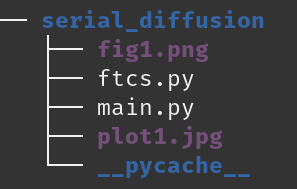
\includegraphics[width=0.3\textwidth]{figures/serial_dir1.png}
    \caption{Contents within serial directory before and after running \texttt{main.py}}
    \label{fig:Serialdir}
\end{figure}
% \vspace{-0.5cm}
The user inputs are intialized as:
\begin{lstlisting}[language=Python]
L = 5
T = 2
h = (2*L)/223 # or (2*L)/707
tau = 0.001 # or 0.0001
\end{lstlisting}

\subsection{Results}
\label{subsec:results}
Currently, we are interested in knowing if our implementation is correct. Fortunately, for our 1D problem, \autoref{eq:De}, there exists an analytical solution \cite{paper}:
\begin{equation}
    v(x,t) = \dfrac{1}{2}\left[ \text{erf}\left( \dfrac{1.5 - x}{2\sqrt{Dt}} \right) - \text{erf}\left( \dfrac{-1.5 - x}{2\sqrt{Dt}} \right) \right] 
    \label{eq:An}
\end{equation}
Here, the error-function $\text{erf}(z) = \frac{2}{\pi}\int_{0}^{z}e^{-y^2} \text{d}y$. This error-function can be used in Python through the SciPy library: \texttt{scipy.special.erf()}

To verify our implementation, we can easily plot our solution obtained through the FTCS method against the analytical solution \autoref{eq:An}. Below are both solutions for $v(x,t)$ plotted at different times $t$.

\begin{figure}[H]
    \centering
    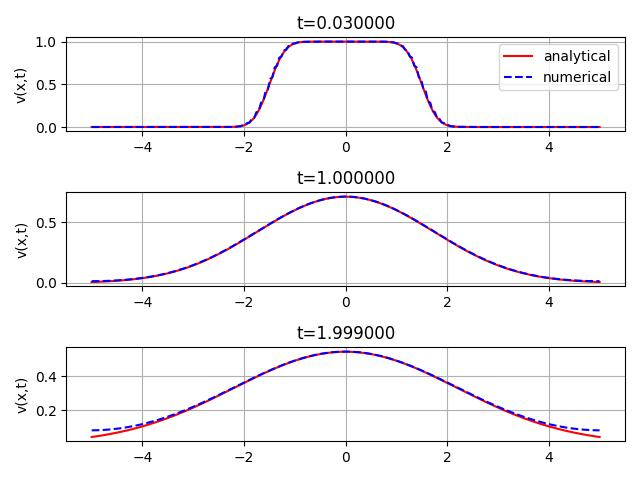
\includegraphics[width=0.6\textwidth]{figures/serial_plot.jpg}
    \caption{Comparison of the solutions obtained analytically (red) and FTCS method (dashed blue)}
    \label{fig:SerialResult}
\end{figure}

We can see in \autoref{fig:SerialResult} that our numerical method performs really well, specially for times $t \ll T$.

The execution times for the numerical method for each case $\tau$ are:
\begin{table}[H]
    \centering
\begin{tabular}{|c|c|c|c|c|}
    \hline
    & $\tau$ & $h$ &  solution matrix \texttt{V} & execution time $[s]$ \\
    \hline
    case 1 & $1\times10^{-2}$ & 0.0448 & 2000 $\times$ 223 & 5.83 \\
    case 2& $1\times10^{-3}$ & 0.0014 & 20000 $\times$ 707 & 187.27 \\
    \hline
\end{tabular}
\caption{Execution times for each case. The size of \texttt{V} significantly increases with finer $\tau$ and $h$, thus increasing execution times. These programs were executed in the \textbf{stromboli} environment}
\end{table}


